\documentclass[runningheads,a4paper]{llncs}
\usepackage{graphicx}
\graphicspath{ {images/} }

\usepackage{amssymb}
\usepackage{url}
\usepackage{times}
\usepackage{float}
\usepackage[T1]{fontenc}
\usepackage[export]{adjustbox}

\usepackage{graphicx}
\usepackage{color}
\usepackage{soul}  
\usepackage{nameref}  
\usepackage{amsbsy}  
\usepackage{bezier}  
\usepackage{colortbl}  
\usepackage[leqno,fleqn]{amsmath}  
\usepackage{verbatim}
\usepackage{listings}

\usepackage[utf8]{inputenc}


\setcounter{tocdepth}{3}
\newcommand{\keywords}[1]{\par\addvspace\baselineskip
\noindent\keywordname\enspace\ignorespaces#1}

\begin{document}
\mainmatter

\title{Review of Paper: Large Scale Cluster Management at Google with Borg }
\subtitle{Paper Review }
\date{Spring 2018}

\author{Dan Budris, Don Yoo, Kanchan Mohite}

\institute{
Boston University\\ Metropolitan College \\ Computer Science Department \\
 dbudris@bu.edu \\ 
 donggun6@bu.edu \\
% \url{http://www.bu.edu }
}

\maketitle
\begin{abstract}
An industry paper which discusses the inner workings of a powerful, large-scale cluster management system used by Google.  The paper uses experimental evidence to display features of the system such as scheduling, task management and resource reclamation.  We will discuss the main features of the paper, related work, and our criticism of the approach.
\end{abstract}

\keywords{Cluster computing, bin packing, scheduling, cluster management, cloud computing}

\section{Introduction}
\subsection{The Paper}
The paper we are reviewing, "Large Scale Cluster Management at Google with Borg",   has numerous authors, all of whom are researchers, software engineers, and site reliability engineers at Google while they worked on the system.  It was originally presented at EuroSys 2015, a high-level industry conference with a focus on distributed systems.  

It’s an industry paper presenting a detailed look at the system by which Google software is deployed and run across large scale clusters.  It is focused primarily on the mechanisms by which the system schedules, distributes, and manages the submitted tasks; as well as the implementation of fault-tolerance and focus on engineering for failure.

\subsection{The System}
Borg is an extremely powerful distributed system built by Google to allow the distribution of large-scale production and batch workloads in a fault-tolerant and easily-accessible manner.  

It’s allows for heterogeneous underlying compute resources to be pooled together into pools of ‘cores’ and ‘memory’, so that jobs can be scheduled on them and executed by a central ‘borgmaster’, or cluster controller.

Each agent has a ‘borglet’, or agent, which controls the processes on the underlying compute resources, receives jobs, controls their local execution, and reports back when polled by the central master server.

The central system uses a domain specific language which allows users of the system to define the resources and scheduling needs of their job in an extremely descriptive manner; this is then submitted to a central server, which takes care of scheduling and distributing the resources across the cluster.  Each ‘cluster’ is, on average, about 10,000 machines; there are more than a dozen clusters globally.  

\section{Motivation of the Research}
This is an extremely powerful global system.  The underlying hardware to operate at 'Google' scale costs hundreds of millions of dollars.  The engineering for the system is also extremely resource intensive -- i.e. expensive.  So, what is the motivation, from an industry perspective, for the creation of this system?  Money, and leveraging economies of scale in order to more efficiently operate their business.

At the scale that Google operates at, saving 1\% can mean many millions of dollars.  By more efficiently packing tasks onto compute resources, Google can save  millions of dollars and ideally save a lot of operator time and effort, as well as reducing downtime. 

Existing cluster management solutions were not equipped to run at the scale that Google required, so they were required to  devise their own system which can permit the operation of large scale clusters and integration with existing Google workflows.

Finally, developer and user productivity is a strong motivator.  Rather than have each team and group operate their own production and test systems, Google provides an internal platform-as-a-service that teams can deploy onto, using the domain specific language to define their tasks and jobs.  By enhancing developer productivity they are in essence saving money, as well as driving their own core products, through an operational strategy.  

\section{Contributions of the Paper}
The paper being reviewed provides an in-depth experimental analysis which justifies the policy decisions made around how 'Borg' schedules, manages, and monitors the applications it deploys.  This kind of in-depth analysis of such a large-scale system is a contribution in and of itself.  In addition, the paper presents a method for low-latency, fault-tolerant distributed task and systems management, and compelling metrics for evaluating such systems (including 'cell compaction' rather than average utilization.

\section{Substantiation of Claims}
In this section, we'll discuss how the experimental results were obtained,  then walk through the major metrics explore: cell compaction, cell sharing, cell segregation,  the impact of large cells, resource requests and reclamation.  

The experimental results for this paper were obtained by taking months-long traces of running Borg cells (clusters), and then using 'Fauxmaster' a high-fidelity Borgmaster replica, to replay the traces with various policy and configuration changes applied.  The results were then compared across numerous metrics and existing performance to determine the most resource and cost effective manner to operate the system and obtain justification for the existing policy choices. 

\subsection{Cell Compaction}

Cell compaction is the metric by which all of the policies of borg, explained later in this presentation, were evaluated.  Since jobs vary widely in their constraints and features, it was believed that Average Cell Utilization was not an adequate metric.  Load spikes, black swan events, and the execution of low-priority jobs in empty resource space needed to be taken into account in determing the best policies and algorithms.  Instead, this paper focused on ‘cell compaction, and which policies would provide the greatest possibilities of cell compaction given the existing configuration.  Cell compaction is how small a given workload can be packed into a cell based on the policies applied to it.  Greater compaction means more workloads can be loaded into smaller cells, meaning that a smaller percentage of the cell is required the greater the compaction is achieved.  The below policies and algorithms are used to maximize cell compaction and, thus, provide the greatest efficiency and cost-savings.


\subsection{Cell Sharing}

Borg manages about 83\% of entire set of machines that runs prod, non-prod task at the same time. prod is long running service that should never die such as Google search, gmail, google doc.
Non-prod is service that takes couple seconds to several day to complete. Other companies usually use prod(user services) and non-prod(batch jobs) in separate clusters. 
It requires 20~30\% more machines to run separate cluster.
Borg can reduce the number of machines used because it handles most non-prod jobs using unused resources.


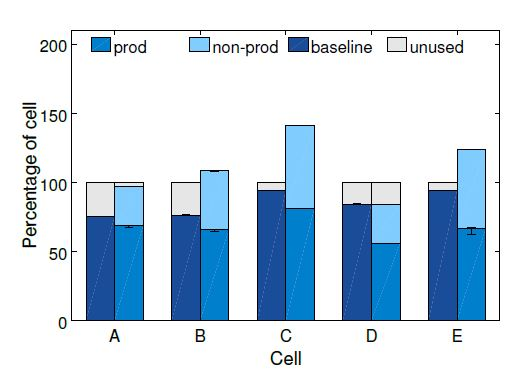
\includegraphics[scale=0.8]{segregation}
from the graph, left one is combined workload and right one is segregated. three of segregated cases are over the cell limit.

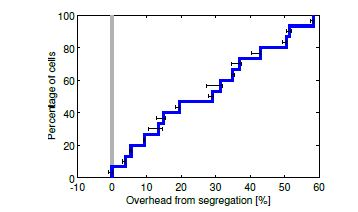
\includegraphics[scale=1.4, left]{cellsharing1}

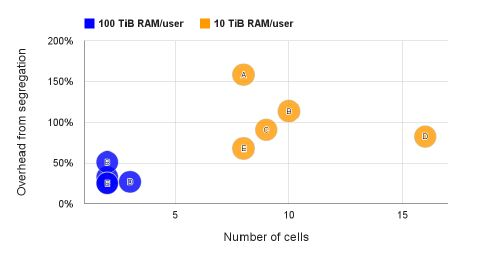
\includegraphics{cellsharing2}
About thousand user share one borg cell. As you see the second graph you can see there are more machines require if users larger than the threshold.
Google also ran CPI (cycle per instruction) test to see if CPU interference is occurring when multiple jobs with different characteristics are running on one machine.
The result is that segregation CPU performance was 3\% better and 1.19 times faster however it is not much significant.

\subsection{Large Cells}

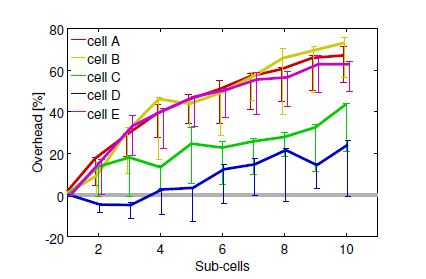
\includegraphics{LargeCell1}

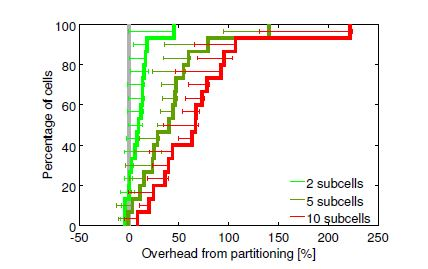
\includegraphics{LargeCell2}

Google builds large cell to reduce number of cells. As result from the graph, it requires more machine if it decides to use smaller cells. 

\subsection{Resource requests and Reclamation}

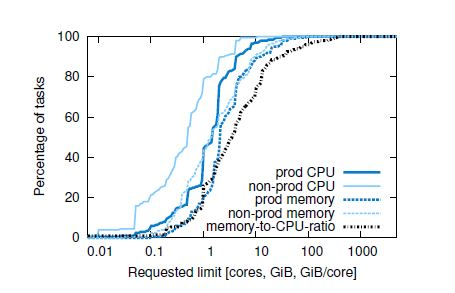
\includegraphics{resourceRequest1}

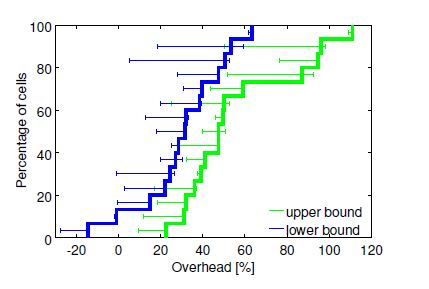
\includegraphics{resourceRequest2}


Borg user can request cpu with mili core, memory and disc with byte unit. If you see the first graph, you can tell user use different size of requirment for cpu and memories.
If borg provide fixed size of container or Virtual Machine, it would require 30~50\% more machines because of overhead.

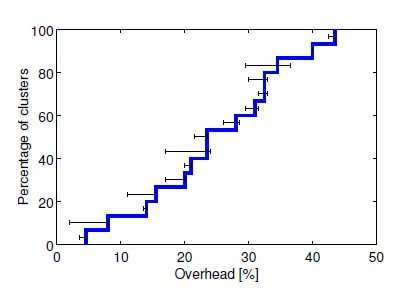
\includegraphics{reclamation1}

 Sometimes user use less than what they requested or use more than what they requested.
Borg use Resource reclamation process to predict how much resource is required for the task and reserve enough space
First reservation is calculated as same requested. Around 300 seconds later it either reduced or expand the size as actual resource is required.

As you see the graph, it require more machine if resource reclamation is not used.

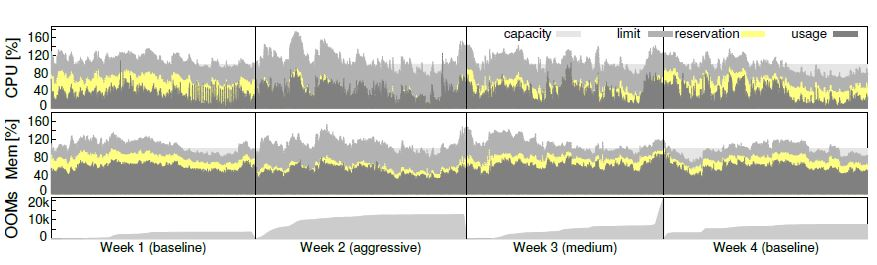
\includegraphics[scale = 0.6]{reclamation2}


Google also test with different reservation algorithm for four weeks to find out what kind estimation would fit the best.
Run baseline for first week, aggressive algorithm for second week, medium algorithm that is between baseline and aggresive and back to baseline.
The result from the graph, second and third week has more OOM(out-of-memory) than baseline.
At the same time, they have more capacity to hold more tasks.
Base on the result, Google choose medium algorithm for resource reclaimation.

\section{Related Work}
While there are numerous contributions of this paper, including the algothrims and systems by which they evaluated the experimental results, our review focused on the other similar cluster management solutions that are comparable to 'Borg'.

\subsection{Other Cluster Managers}
Most web-scale companies have cluster management solutions, most of which are home-grown.  Some of these companies include Microsoft, Facebook, Twitter, and Alibaba.  Most of these systems are proprietary and the details are not available to the public.  

There are numerous other systems that are comparable to Borg.
Only some of these systems are tested and executed at the scale that Borg operates at -- and are mainly operated by web-scale companies, such as Facebook, Microsoft and Alibaba.  We don’t know a lot about them, as they are private, internal systems; the operational efficiency that they provide is a serious competitive advantage.

Kubernetes, OpenShift and Amazon Elastic Container Service offer public platforms to deploy containerized applications onto self-healing clusters.  These systems also offer domain specific languages for deployment and control, packing and scheduling algorithm choice and control, reporting and self-healing. 

Kubernetes is a major successor of Borg, built by Google, and directly draws on the lessons learned and technology developed for Borg, applied to an open-source project.  

\subsection{Kubernetes}
Kubernetes is a large, open-source project which was derived directly from Borg by Google engineers and then made available to the wider public.  The system provides many of the cluster-management tools discussed in the previous sections, while also allowing for important distinctions between tasks that were not available in in Borg.  It is viewed by the paper as one of the most important related pieces of work.

Currently Kubernetes is the largest open-source project on Github, with thousands of contributors, and is used to operate large-scale compute clusters around the world.

\section{Conclusion}

\subsection{Strengths of Approach}
This paper provided a succinct but complete description of complete system and its implications, with a detailed architectural overview as well as experimental results justifying the decisions. 

Detailed explanation of policy decisions (e.g. running prod and non-prod together), and how they relate back to the motivation (reducing operational costs and allowing for sufficient scale).

Resource allocation methodology well explained and argued, with solid empirical result to back it up.  Each step of the way this paper provided detailed experimental results to back up their decisions and careful explanations of the importance of those results.  

\subsection{Weaknesses of Approach}
The experimental results focus almost totally on the resource allocation and scheduling; it would have been powerful to see more experimental and objective results regarding the usage behavior of end-users.

Experimental results based off of ‘months long trace’ is not explained, methodology unclear.  While the use of the 'Fauxmaster' is in fact explained, it would be very meaningful to get a greater level of detail on how the monitoring works.

Some concepts are not adequately explored -- for example, “link shards” are discussed but never actually explained as an architectural concept.  Additonally, the distributed storage systems is not explained.  It can be reasoned that the distributed storage systems underlying Borg are sufficiently large and complex to warrent a study all their own and addressing them in this paper would have been tangential.  


\bibliographystyle{plain}
\bibliography{literature}
\end{document}
